\newpage
\section{Design pattern utilizzati}

\subsection{Abstract Factory}
L'\textbf{\textit{Abstract Factory}} è un design pattern creazionale e fornisce un'interfaccia per creare famiglie di prodotti, senza dover esplicitare il nome concreto delle classi a cui si riferisce. In questo modo, si permette che un sistema sia indipendente dall'implementazione degli oggetti concreti e che il client, attraverso l'interfaccia, utilizzi diverse famiglie di prodotti. Quindi, il client conosce solo l’interfaccia per creare le famiglie di prodotti, ma non la sua implementazione concreta.
L’\textit{Abstract Factory} è costituito da 5 elementi:
\begin{itemize}
	\item \textbf{AbstractFactory}: dichiara un'interfaccia per le operazioni che crea oggetti product astratti;
	\item \textbf{ConcreteFactory}: implementa le operazioni per creare oggetti concreti product di AbstractProduct. Per garantire che nel sistema esiste un’unica istanza di ciascuna ConcreteFactory, è buona norma definire ciascuna di esse come \textit{Singleton};
	\item \textbf{AbstractProduct}: interfaccia che definisce la struttura base dei product che la factory può instanziare;
	\item \textbf{ConcreteProduct}: nel sistema possono essere creati n ConcreteProduct, ciascuno dei quali dovrà implementare l’interfaccia AbstractProduct;
	\item \textbf{Client}: utilizza l’AbstractFactory per generare i prodotti concreti all’interno del sistema.
\end{itemize}

\begin{figure}[H]
	\centering
	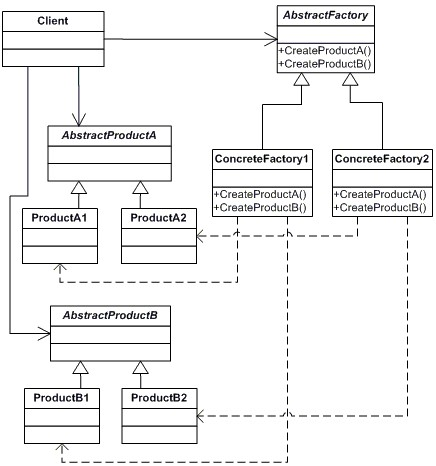
\includegraphics[width=0.5\linewidth]{IMG/abstract-pattern}
	\caption{Design pattern Abstract Factory}
\end{figure}

I punti di forza di questo design pattern sono:
\begin{itemize}
	\item Isola i client dall’implementazione delle classi concrete;
	\item Rafforza il raggruppamento di prodotti in famiglie;
	\item Rende possibile interscambiare facilmente le famiglie di prodotti, perché ogni factory concreta genera una famiglia di prodotti.
\end{itemize}

\subsubsection{Campo di utilizzo}
Nel sistema realizzato, il design pattern \textit{Abstract Factory} verrà utilizzato per rendere il sistema indipendente dalla creazione delle classi concrete ed essere aperto all’estensione tramite la definizione di nuovi tipi.


\subsection{Singleton}
Il \textbf{\textit{Singleton}} è un design pattern creazionale che ha lo scopo di garantire che venga creata una e una sola istanza di una determinata classe, e di fornire un punto di accesso globale a tale istanza.
Gli elementi caratteristici fondamentali per l'implementazione di questo pattern sono due:
\begin{itemize}
	\item Un costruttore privato, per evitare che la classe possa essere istanziata arbitrariamente;
	\item Un metodo statico per accedere alla singola istanza.
\end{itemize}
\begin{figure}[H]
	\centering
	
\includegraphics[width=0.4\linewidth]{IMG/singleton_pattern}
	\caption{Design pattern Singleton}
\end{figure}

I punti di forza di questo design pattern sono:
\begin{itemize}
	\item L'accesso controllato all'istanza;
	\item \MakeUppercase{è} possibile consentire più istanze, sempre in modo controllato.
\end{itemize}

\subsubsection{Campo di utilizzo}
Ogni servizio in AngularJS è un \textit{Singleton}, perchè ogni servizio è istanziato non più di una volta. In \progetto\ saranno presenti dei servizi per gestire le interazioni tra la web app e i database contenenti i dati.
Il design pattern \textit{Singleton} è stato utilizzato anche per il back-end della piattaforma, infatti ogni microservizio realizzato in Jolie è istanziato solo una volta all'avvio e rimane in attesa di input per operare sul database e fornire risultati al servizio chiamante del front-end. 


\subsection{Facade}
Il \textbf{\textit{Facade}} è un design pattern strutturale che permette, attraverso un'interfaccia più semplice, l'accesso a sottosistemi che espongono interfacce complesse e molto diverse tra loro, nonché a blocchi di codice complessi.
Questo rende una libreria più facile da capire, usare e testare, inoltre permette di diminuire le dipendenze tra sottosistemi senza nascondere le funzionalità di basso livello.

\begin{figure}[H]
	\centering
	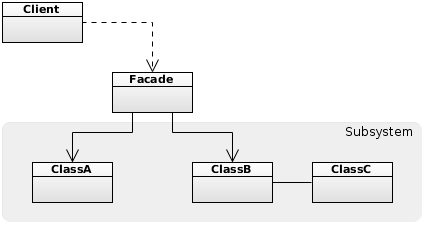
\includegraphics[width=0.7\linewidth]{IMG/facade_pattern.png}
	\caption{Design pattern Facade}
\end{figure}

I punti di forza di questo design pattern sono:
\begin{itemize}
	\item Nascondere la complessità dell'operazione all'interno di un sistema complesso;
	
	\item Fornisce un'interfaccia semplificata al client.
\end{itemize}

\subsubsection{Campo di utilizzo}
Nella parte front-end dell'applicazione, il design pattern Facade viene utilizzato nel file principale \textit{app.js}. Questo file definisce le routes dell'applicazione e viene utilizzato per associare
un URL alle varie \textit{view} dell'applicazione.\\
All'interno del file è utilizzata la funzione  \textit{\$locationProvider} e \textit{\$routeProvider} che gestiscono il routing e specificano quale pagina utilizzare in caso non venga specificato l'URL.\\
Inoltre, il pattern Facade viene utilizzato nella parte di back-end dall'API Gateway quando un utente sviluppatore inserisce un microservizio sulla piattaforma. Infatti, esso può essere composto da un numero arbitrario di interfacce e sarà compito del gateway fornire ai clienti del marketplace un'interfaccia unificata, in modo da rendere user friendly l'utilizzo.


\subsection{Decorator}
Il \textbf{\textit{Decorator}} è un design pattern strutturale che permette di aggiungere dinamicamente nuove responsabilità ad un oggetto. In questo modo, si possono estendere le funzionalità di oggetti particolari senza coinvolgere
complete classi (senza dover utilizzare il subclassing).

\begin{figure}[H]
	\centering
	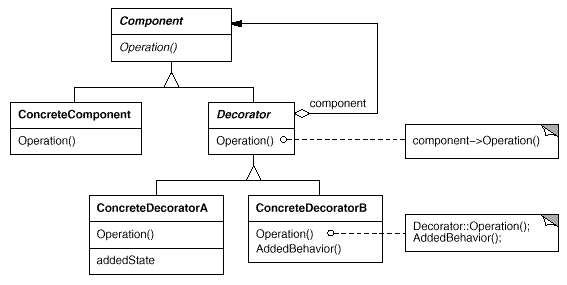
\includegraphics[width=0.7\linewidth]{IMG/decorator_pattern.png}
	\caption{Design pattern Decorator}
\end{figure}

Questa tecnica si applica quando:
\begin{itemize}
	\item Occorre aggiungere funzionalità dinamicamente ad un oggetto in modo	trasparente;
	
	\item Si vogliono "circoscrivere" le funzionalità;
	
	\item Non è possibile estendere una classe per subclassing.
\end{itemize}

\subsubsection{Campo di utilizzo}
Il pattern Decorator viene utilizzato nella parte di back-end dall'API Gateway quando avviene la richiesta di utilizzo di un microservizio da parte di un utente cliente. Il gateway deve aggiungere dinamicamente (decorare) delle informazioni alla richiesta del cliente, che ha a disposizione la sola interfaccia del microservizio target. I dati aggiunti servono per il monitoring dei dati di SLA (Service Level Agreement) e per la parte di comunicazione vera e propria con il microservizio Jolie (location e protocol).